Der icore ist ein rekonfigurierbarer Prozessor \comment{(Cite Missing)}, das bedeutet er besitzt neben den klassischen Komponenten
eines Prozessors noch eine zur Laufzeit konfigurierbare Einheit aus Hardwarebeschleunigern. Aktuell ist er vollständig auf einer Xilinx VC-707 FPGA (siehe Abschnitt \ref{sec:fpga}) implementiert.
Als Grundlage dient ein modifizierter Leon3-Kern, ein 7-Stufen-Pipeline-Prozessor basierend auf der SPARC-V8-Architektur \comment{(Cite Missing)}.
Er wird erweitert um eine sogenannte \textbf{Reconfigurable Fabric}, einen Container für fünf Beschleunigerblöcke mit Anbindung an Speicher und Registerdatei.
Wie genau diese Fabric aufgebaut ist und wie sie funktioniert schauen wir uns in Abschnitt \ref{sec:icore_arch} an.
Vorher wollen wir uns aber erstmal überlegen wofür rekonfiguruerbare Prozessoren eigentlich gut sind.
\section{Rekonfigurierbare Prozessoren}
Herkömmliche Prozessoren verfügen über einen mehr oder weniger komplexen Befehlssatz, der es ihnen erlaubt jede beliebige Berechnung durchzuführen,
indem die gewünschte Rechenoperation in mehrere vom Befehlssatz unterstützte Operationen aufgeteilt wird. Dadurch sind sie extrem flexibel.
Für rechenintensive Aufgaben, bei denen komplexere Operationen sehr oft ausgeführt werden müssen, ist dieser Ansatz jedoch nachteilig,
da der Prozessor viel Zeit benötigt, um diese komplexen Operationen zu berechnen. Um dem Abhilfe zu verschaffen, wird spezializsierte Hardware
wie zum Beispiel Grafikkarten, Netzwerkkarten oder FPGAs eingesetzt, die besonders effizient eine bestimmte Art von Aufgabe erfüllen.
Durch die fortschreitende Digitalisierung und Vorstöße in Bereichen wie der Industrie 4.0 oder dem Internet der Dinge (IoT) wächst der Bedarf an Kleinstrechensystemen,
die für den konkreten Anwendungszweck spezielle Aufgaben übernehmen können. Diese müssen vor allem energieeffizient, klein und günstig in der Produktion sein
und müssen dabei trotzdem auch in der Lage sein komplexere Aufgaben teilweise sogar in Echtzeit erfüllen zu können.
Ein rekonfigurierbarer Prozessor bietet hier die Vorteile der hohen Flexibilität eines normalen Prozessors und verbindet sie mit der hohen Spezialisierbarkeit von FPGAs,
indem er mehrere kleine Blöcke an vom Entwickler konfigurierbare Logikblöcke bereitstellt, die mit speziellen Prozessorinstruktionen gesteuert werden können.
Auf diese Weise können auch sehr spezielle Anwendungen von Off-The-Shelf Hardware erfüllt werden, was die Produktionskosten gegenüber Spezialanfertigungen,
sowie den Energieverbrauch und den Bedarf an Rechenleistung gegenüber klassischen Prozessoren reduziert.

\subsection{FPGA}
\label{sec:fpga}
\begin{figure}
    \center
    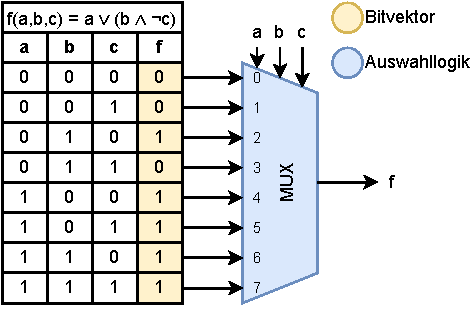
\includegraphics{images/LUT.pdf}
    \caption{Implementierung einer dreistelligen Funktion durch einen Lookup Table}
    \label{fig:fpga_lut}
\end{figure}
\textbf{Field Programmable Gate Arrays} (FPGAs) sind integrierte Schaltkreise, die von sich aus keine genaue Funktion implementieren. Stattdessen muss erst eine Schaltung "geladen" werden.
Dabei macht man sich zu Nutze, dass eine n-stellige boolsche Funktion durch einen $2^n$-Bit Vektor codiert werden kann. In Abb. \ref{fig:fpga_lut} ist zum Beispiel die Funktion $f = A \vee (B \wedge \neg C)$ dargestellt.
Der 8-Bit Ergebnisvektor wird in SRAM-Speicherzellen gehalten und durch einen 8-zu-1-Multiplexer kann mit $A$, $B$ und $C$ das entsprechende Ergebnisbit ausgewählt werden. Diese Schaltung wird Lookup Table (LUT) genannt.
Mehrere solcher Lookup Tables werden zusammen mit anderen Komponenten wie zum Beispiel Flip-Flops oder Recheneinheiten wie Full-Addern zu sogenannten \textbf{Configurable Logic Blocks} (CLBs) zusammengefasst, im Folgenden auch Logikblöcke genannt.
Logikblöcke sind bereits sehr vielseitig, aufgrund der festen Anordnung ihrer Komponenten jedoch immer noch stark eingeschränkt. Um dem entgegen zu wirken sind die Logikblöcke untereinander mit einem flexiblen
und ebenfalls konfigurierbaren Verbindungsnetz verbunden. Auf diese Weise kann jede beliebige Funktion realisiert werden, sofern genug Logikblöcke zur Verfügung stehen.
Neben den normalen Logikblöcken stellen FPGAs typischerweise auch noch andere Komponenten bereit, die etwas speziellere Funktionen realisieren, die oft benötigt werden
und die sehr viel Platz benötigen, wenn mit Logikblöcken implementert. Dazu gehören unter anderem \textbf{Digital Signal Processors} (DSPs), sie stellen Funktionen bereit, die zur Signalverarbeitung benötigt werden,
und \textbf{Block RAM} (BRAMs), die ähnlich wie klassischer RAM in der Lage sind eine große Menge Daten zu speichern.
FPGAs haben gegenüber Mikroprozessoren den großen Vorteil, dass alle Funktionen, die von den Logikblöcken realisiert werden, gleichzeitig und kontinuierlich berechnet werden.
Auf diese Weise kann eine enorme Beschleunigung gegenüber einer reinen Software-Implementierung erzielt werden, da der Prozessor alle Berechnungen nacheinander durchführen muss.

\section{icore-Architektur}
\begin{figure}
    \center
    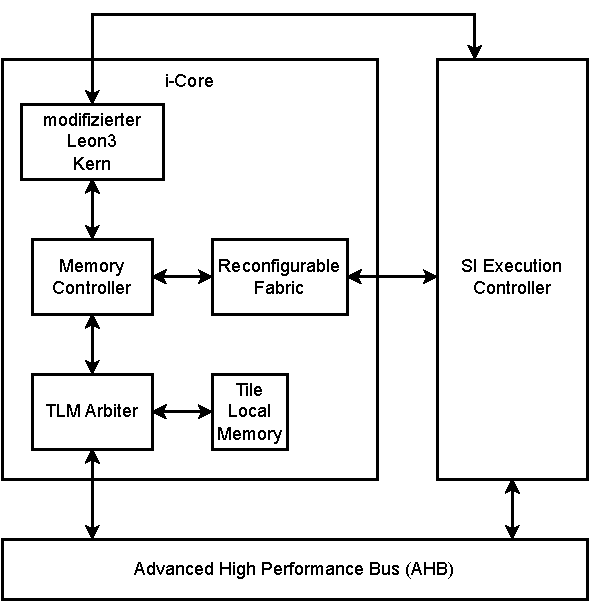
\includegraphics{images/Icore_Arch.pdf}
    \caption{Aufbau des icore mit Ausführungskontrolle und Reconfigurable Fabric (\comment{Nachbildung aus (Cite missing, [3])})}
    \label{fig:icore_arch}
\end{figure}
\label{sec:icore_arch}
Der icore ist ein Multicoreprozessor, der vollständig auf einer FPGA implementiert ist. Als Hardware wird ein Xilinx VC 707 Board verwendet.
Es handelt sich um einen heterogenen Prozessor, seine Kerne sind also unterschiedlich gebaut. Während zwar alle Kerne auf dem Leon3 basieren,
verfügt der Primärkern, wie in Abb. \ref{fig:icore_arch} über die \textit{Reconfigurable Fabric}.
Diese Fabric enthält fünf zur Laufzeit rekonfigurierbare Blöcke, die sogenannten \textbf{Atome}, die zur Hardwarebeschleunigung verwendet werden können.
Der Primärkern verfügt außerdem noch über einen 1MB großen \textit{Tile Local Memory} (TLM), der mit dem \textit{Memory Controller} über ein 256 Bit breites Interface verbunden ist.

\subsection{Reconfigurable Fabric}
\begin{figure}
    \center
    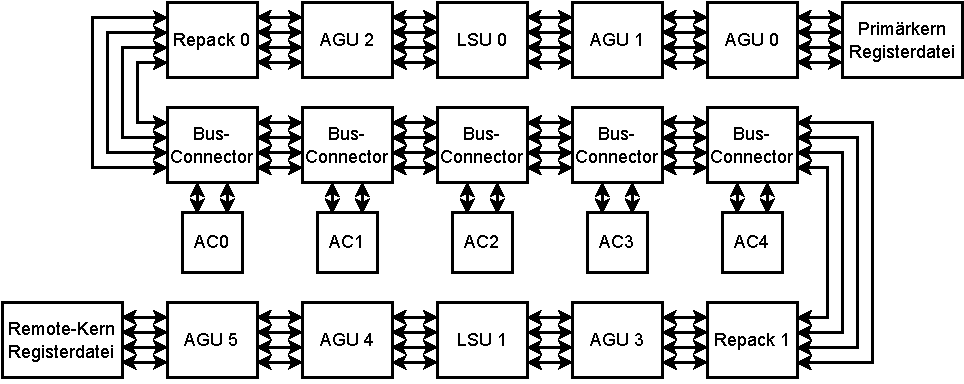
\includegraphics{images/Icore_Fabric.pdf}
    \caption{Aufbau der Reconfigurable Fabric}
    \label{fig:icore_fabric}
\end{figure}
Die \textit{Reconfigurable Fabric} enthält fünf Atomcontainer (AC0 bis AC4), die zur Laufzeit rekonfiguriert werden können und in die die Beschleuniger geladen werden.
Jedes Atom hat eine Größe von 1600 LUTs, die den Beschleunigern zur Verfügung stehen. Über einen Bus-Connector sind die Atome über eine 2 Lane breite Schnittstelle
an einen 4 Lane breiten Bus angebunden (eine Lane ist ein Vollduplexkanal mit einer Breite von 32 Bit). Welche Kanäle den Atomen als Ein- und Ausgabe dienen,
wird von den VLCWs der Spezialinstruktion bestimmt (siehe Abschnitt \ref{sec:special_instruction}). Der Bus ist segmentiert, das heißt es können auch mehrere Kommunikationen über den gleichen Kanal stattfinden,
solange sich die Kommunikationspfade nicht physisch überlappen. Neben den Atomcontainern verfügt die \textit{Reconfigurable Fabric}
noch über weitere Komponenten wie \textit{Load-Store-Units} (LSUs), mit denen Daten aus dem TLM oder dem RAM gelesen oder geschrieben werden können. Jede LSU besitzt eine 128 Bit Anbindung mit dem TLM,
mit dem die LSU mit geringer Latenz eine große Menge Daten verarbeiten kann. Um die gelesenen Daten zu halten, stehen den LSUs jeweils vier Puffer it jeweils 128 Bit zur Verfügung.
Mit Hilfe von \textit{Address-Generation-Units} (AGUs) können verschiedene Zugriffsmuster für die LSUs generiert werden.
Zuletzt gibt es noch die \textit{Repack Units} mit denen Daten auf dem Bus kombiniert werden können. Wir werden sie nicht weiter benötigen, deshalb seien sie hier nur der Vollständigkeit halber kurz erwähnt.
All diese Komponenten sind ebenfalls mit dem Bus verbunden. An den Enden des Busses werden die Register des Prozessors bereitgestellt, sodass die Fabric auf bis zu vier Argumente zugreifen kann.
Die genaue Anordnung der Komponenten ist in Abbildung \ref{fig:icore_fabric} dargestellt.

\subsection{Spezialinstruktionen}
\label{sec:special_instruction}
Der Prozessor stellt Spezialinstruktionen (SIs) bereit, die von Programmen benutzt werden, um die Beschleuniger zu verwenden.
Taucht eine solche Spezialinstruktion im Programmcode auf, wird die Pipeline des Prozessors angehalten und, falls notwendig,
die für den Beschleuniger benötigten Atome konfiguriert. Über den \textit{SI Execution Controller} (siehe Abschnitt \ref{sec:si_exec_ctl})
wird dann die Abarbeitung durch den Beschleuniger durchgeführt. Nachdem die Abarbeitung abgeschlossen ist, wird dann die Kontrolle wieder an den Prozessorkern übertragen
und die Pipeline wird neugestartet. Dabei ist noch anzumerken, dass die \textit{Reconfigurable Fabric} zwar nur im Primärkern implementiert ist,
die anderen Kerne jedoch trotzdem die Beschleuniger verwenden können, indem sie über den AHB den \textit{SI Execution Controller} ansprechen (siehe Abb. \ref{fig:icore_arch}), der die \textit{Reconfigurable Fabric} verwaltet.

\subsection{SI Execution Controller}
\label{sec:si_exec_ctl}
Die Spezialinstruktionen sind mit VLCWs mikroprogrammiert. Wird ein Beschleuniger geladen wird auch der Mikrocode für den Beschleuniger in den \textit{Execution Controller} geladen.
Dieser hat die volle Kontrolle über die \textit{Reconfigurable Fabric} und kontrolliert mit Hilfe der VLCWs ihre Komponenten.
Jedes VLCW definiert dabei einen Kontrollschritt, die der Reihe nach abgearbeitet werden. Für die Atome werden von einem VLCW die Anbindung der Eingabe- und Ausgabelanes an den Bus bestimmt sowie ein 6 Bit Kontrollvektor.
Die Funktion des Kontrollvektors kann im Atom beliebig realisiert werden. Für die LSUs wird bestimmt welche AGU zur Adressgenerierung verwendet werden soll,
welche Puffer für die Lese-/Schreiboperation verwendet werden sollen und welche Daten aus dem Puffer an den Bus angelegt werden sollen bzw. vom Bus in den Puffer übernommen werden sollen.
Für die AGUs wird der Betriebsmodus über die VLCWs bestimmt. Es gibt sowohl Betriebsmodi für rein statische Zugriffsmuster, die vollständig über die VLCWs bestimmt werden, als auch dynamische Modi,
bei denen das Zugriffsmuster über Parameter direkt vom Datenbus bestimmt wird. Für jede Spezialinstruktionen stehen insgesamt \comment{256} VLCWs zur Verfügung.
\comment{Um auch Programme zu realisieren, die länger als 256 Kontrollschritte sind, sind auch rudimentäre Schleifen in dem Mikrocode mögich.}

\section{Erweiterung Dynamic Execution}
Um auch einen dynamischen Kontrollfluss innerhalb des VLCW-Mikrocodes zu ermöglichen, wie zum Beispiel Schleifen, die von einem Laufzeitparameter abhängen,
verwenden wir eine von Sascha Hering entwickelte Erweiterung der VLCWs \comment{(Cite missing, [3])}. Die Atomcontainer werden mit \comment{zwei} weiteren Ausgabebits ausgestattet.
Diese können vom den Atomen des Beschleunigers beliebig implementiert werden. Um nun Sprünge realisieren zu können, werden die VLCWs um einen neuen Kontrollabschnitt erweitert.
Dieser kann benutzt werden, um Zählervariablen für Schleifen zu setzen oder Sprünge anhand von diesen Zählern durchzuführen. Es sind jedoch auch Sprünge möglich,
Die nur bei bestimmten Mustern der neuen Ausgabebits der Atome genommen werden. Hierzu lässt sich im VLCW mit einer Bitmaske codieren welche Atom Container betrachtet werden sollen,
ob die Bedingung für alle oder nur für ein Atom erfüllt sein muss, welche Vergleichsoperation auf dem \comment{Kontrollvektor} durchgeführt werden soll und
zu welcher VLCW gesprungen werden soll. Diese Erweiterung ist für die Realisierung von Hashfunktionen besonders interessant, da die Eingabelänge für die Berechnung völlig variabel ist
und so immer zur Laufzeit bestimmt werden muss, wie oft die zugrundeliegende Funktion berechnet werden muss. Ohne diese Erweiterung wäre es nicht möglich die vollständige Berechnung innerhalb einer einzigen
Spezialinstruktion durchzuführen, sondern der dynamische Teil müsste in Software implementiert werden und es müsste nach jeder Iteration des beschleunigers das Zwischenergebnis gespeichert werden was,
wie wir später bei der Implementierung sehen werden, zu starken Leistungseinbußen führen würde.